\iffalse
\bibliography{reference/refs}
\fi


\chapter{Face De-Identification in Videos}
\label{chap:FDvideos}

	Different with the previous chapter that focuses on face 
	de-identification about still images, this chapter proposes 
	an approach to de-identify the faces in every frame of a 
	video. Besides the problems mentioned in the previous chapter,
	one more challenge in face de-identification about videos is
	to keep the de-identified person constant. Since a person
	would appear in the adjacent frames of a video, it would be
	strange if the de-identified person changes between frames.  


	This chapter would introduce the overview of our proposed algorithm firstly,
	and then describe the details of our approach in three steps. Section \ref{sec:pre_processing}
	demonstrates the build up of the AAM and the higher-order tensor for 
	coefficients. Section \ref{sec:oneFrame} shows the face de-identification process for a single 
  	video frame. Section \ref{sec:video} introduces how to extend the face de-identification 
  	to other frames in the video. In the following, we summarize the algorithm in section 
  	\ref{sec:video_summary}. Finally, the related experiments are shown to prove the effectiveness
  	of our proposed algorithm.

\section{Algorithm Overview}
\label{sec:algorithm}
	Numbers of face de-identification algorithms have been demonstrated
	in the previous chapter. It indicates that only replacing the original
	face region with a natural looking face could make the de-identified
	image readable to humans. With the purpose of keeping balance between
	privacy protection and data utility preservation as the key problem,
	the de-identification algorithm for videos also uses face substitution.
	Compared to the alogrithms for still images, a video is consisted of
	a set of adjacent frames. It is not workable to simply process the video
	frame by frame as the still images. Because one person appears in adjacent
	frames should still be de-identified as the same person. 

	To achieve this goal, we use AAM and tensor HOSVD to process one frame
	and then all the other frames with the same way. To make it clear, a flow 
	diagram is illustrated as figure \ref{fig:video_diagram}.

  	\begin{figure}[!htb]
	    \centering
		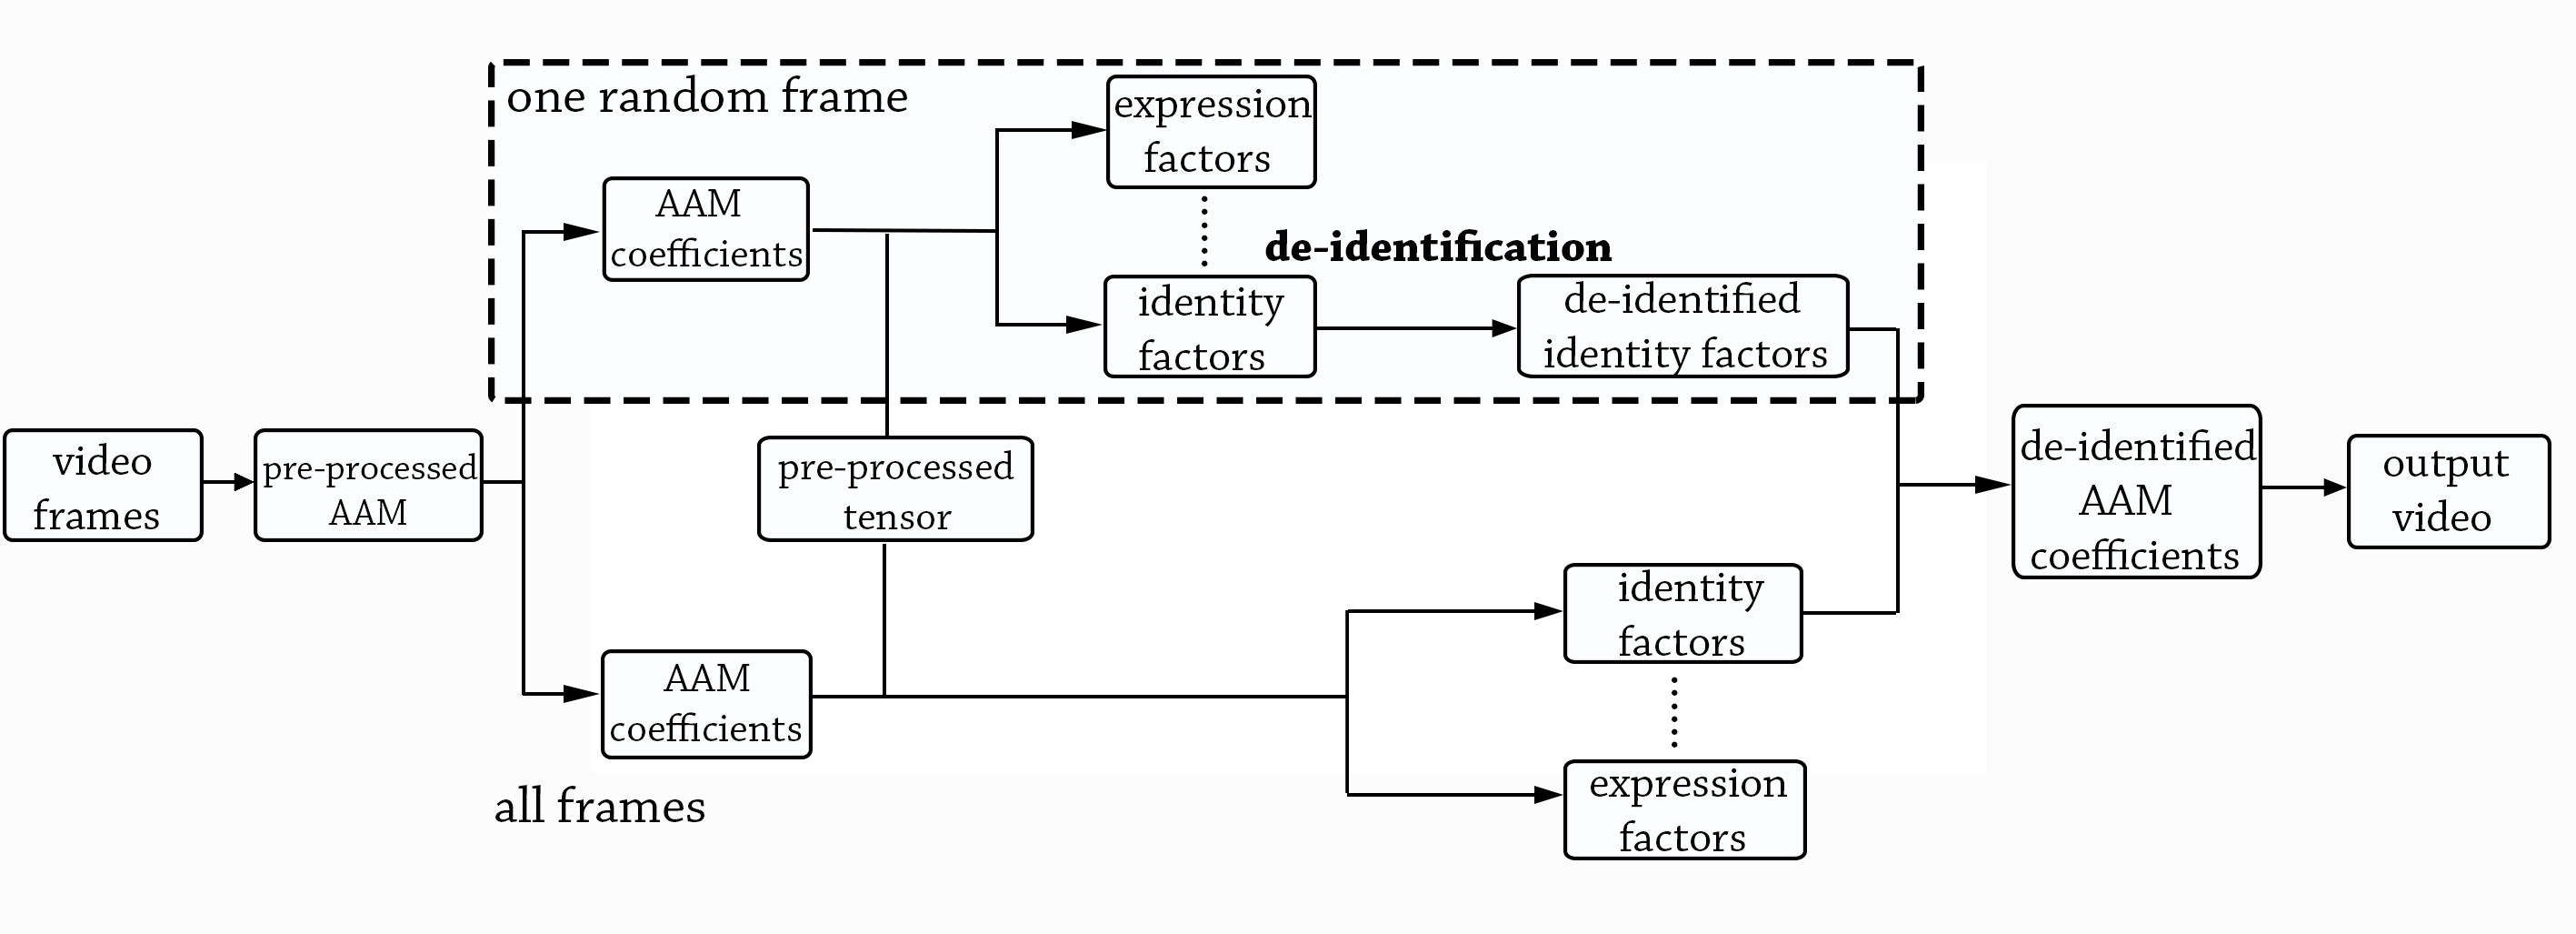
\includegraphics[scale = 0.6]{figure/VideoDiagram}
	    \caption{Flow diagram of the proposed algorithm. Dashed box is the de-identification process for one frame.}
	    \label{fig:video_diagram}
	\end{figure}
  	
  	As shown in the diagram, a video is considered as a set of frames. The face region in each frame is represented by
  	a AAM which is constructed by some selected images. These images are from different people and each person has 
  	multiple images that contains different expressions, poses or skin colors. The AAM projects a face image into an 
  	image space so that each image is converted into a set of coefficients.
  	It has been proved that a face image could be decomposed into multiple dimensions, such as $identity$ factors, 
  	$expression$ factors, $pose$ factors, etc. \cite{VasilescuT03,TPAMI09,Feng12} using tensor analysis.
  	Therefore, we then build up a higher-order tensor based on image coefficients. 
  	Based on the theory of HOSVD, a $n$-mode tensor is obtained from the outer product of a $n$-mode core tensor and $n$ 
  	square matrixes (see details in section 3.1). The AAM coefficients of the image could be decomposed into $identity$ 
  	factors and other types of non-identity factors by the core tensor and the square matrixes. Finally, during the 
  	video de-identification, one of the video frames is picked out randomly. We blend its $identity$ factors with $k$ other $identity$ 
  	factors from different persons to form a set of factors, which we call it as the de-identified $identity$ factors. 
  	For all the other frames in the video, we also decompose the AAM coefficients into $identity$ factors and 
  	other ones, then reconstruct the video frames using the de-identified $identity$ factors and their own other non-identity factors.



	\section{Pre-processing}	
	\label{sec:pre_processing}
	In order to get natural de-identified images, we build an AAM for image representation in advance.
	In this step, an image is projected into a vector space so that it is represented by a set of coefficients \cite{Matthews_04}. 
	Generally, the model
	is built up in two levels: shapes and appearances. Since the shape keeps more information about expressions and the appearance is more
	related to identity information, we focus only on the appearance model. In detail, the pixels within face region are listed as a vector, 
	then a set of images construct a matrix of the pixels which. Lastly, a vector space is formed according to the PCA results
	of the pixel matrix. 

	Following the symbols defined before, the texture of one image is represented as:
	\begin{align}
		\label{equ:aam}
		\begin{split}
			A = A_0 + \sum_{i=1}^{n}\lambda_i * A_i,
		\end{split}
	\end{align}
	where $A_0$ is a mean texture, $A_i$ is a result vector from PCA computation, $\lambda_i$ is the coefficients of the image.

	To decompose the coefficients of an image into $identity$ factors and other factors, a higher-order tensor is required.
	We build up a tensor, called $\mathcal{C}$, of the coefficients according to the types of data utility, such as 
	expressions, poses. Suppose the coefficients of a image $\bf{c} \in R^{n \times 1}$ and two types of data
	utility need to be preserved: $4$ types of expressions and $3$ types of poses, the coefficient tensor should be $\mathcal{C} \in 
	R^{4 \times 3 \times n}$. Each dimension of $\mathcal{C}$ subjects to expressions, poses coefficients \cite{VasilescuT03,Feng12}. 

	According to the HOSVD \cite{Lathauwer00,Kolda09}, any tensor $\mathcal{C} \in R^{i_1 \times i_2 \times ... \times i_n}$ could be decomposed
	as:
	\begin{align}
		\label{equ:hosvd_1}
		\begin{split}
			\mathcal{C} = \mathcal{C}_{core} \times_1 U_1 \times_2 U_2 ... \times_n U_n,
		\end{split}
	\end{align}
	where $\mathcal{C}_{core}$ is a core tensor whose size is the same as $\mathcal{C}$, $U_i$ is the left part in SVD results 
	of corresponding mode-$i$ flattening of $\mathcal{C}$.


	\section{Face De-Identification In One Frame}
	\label{sec:oneFrame}
	The face de-identification in videos is processed frame by frame. This part shows the process in one frame that is randomly
	selected. The AAM coefficients of the selected frame would be decomposed and the expected result is a set of de-identified 
	$identity$ coefficients.

	Suppose we have a set of images containing $n_1$ identities, $n_2$ expressions and each of them is represented by a 
	$n_3 \times 1$ vector, the pre-processed tensor is $\mathcal{D} \in R^{n_1 \times n_2 \times n_3}$. 
	A basis tensor about one expression is \cite{TPAMI09} : 
	\begin{align}
		\label{equ:base_tensor}
		\begin{split}
			\mathcal{D}_{base} = \mathcal{D}_{core} \times_1 U_1 \times_2 U_2(i,:) \times_3 U_3 ,
			% \mathcal{C} = \mathcal{C}_{core} \times_1 U_1 \times_2 U_2 ... \times_n U_n,
		\end{split}
	\end{align}
	where $\mathcal{D}_{base} \in R^{n_1 \times n_3}$, $U_1 \in R^{n_1 \times n_1}$, $U_3 \in R^{n_3 \times n_3}$,
	$D_{core} \in R^{n_1 \times n_2 \times n_3}$ and $1 \le i \le n_2$. $\mathcal{D}_{base}$ is a basis tensor about
	the $i$-th expression in $U_2$, which means that the product result of $\mathcal{D}_{base}$ and different $identity$
	coefficients could produce variants images with the $i$-th expression. Inferred from this example, the basis tensor 
	of a general tensor, $\mathcal{C} \in R^{n_1 \times n_2 \times n_3 ... \times n_m}$, is:
	\begin{align}
		\label{equ:general_base_tensor}
		\begin{split}
			\mathcal{B}_{base} = \mathcal{C}_{core} \times_1 U_1 \times_2 U_2(i_2,:) \times_3 U_3(i_3,:) ... \times_{m-1} U_{m-1}(i_{m-1},:) \times_m U_m ,
			% \mathcal{C} = \mathcal{C}_{core} \times_1 U_1 \times_2 U_2 ... \times_n U_n,
		\end{split}
	\end{align}
	where the first dimension of $\mathcal{C}$ is $identity$, the $m$-th dimension is AAM coefficients and $1 \le i_j \le n_j$. 
	Therefore, the AAM coefficients of an image, $img \in R^{n_m \times 1}$, is:
	\begin{align}
		\label{equ:img_representation}
		\begin{split}
			img = \mathcal{C}_{core} \times_1 {\bf c}_{idj}^T*U_1 \times_2 U_2(i_2,:) \times_3 U_3(i_3,:) ... \times_{m-1} U_{m-1}(i_{m-1},:) \times_m U_m ,
			% \mathcal{C} = \mathcal{C}_{core} \times_1 U_1 \times_2 U_2 ... \times_n U_n,
		\end{split}
	\end{align}
	where ${\bf c}_{idj}$ is the $identity$ factors.

	With $B \in R^{i_1 \times i_n}$ being the stack matrix of the $\mathcal{B}_{base}$ in its first dimension, the $identity$ coefficients of
	an image could be represented as:
	\begin{align}
		\label{equ:identity_coeff}
		\begin{split}
			{\bf{c}}_{idj}^T = B^{-1} * img.
			% \mathcal{C} = \mathcal{C}_{core} \times_1 U_1 \times_2 U_2 ... \times_n U_n,
		\end{split}
	\end{align}
	Therefore, the reconstructed AAM coefficients of this frame is:
	\begin{align}
		\label{equ:img_recon}
		\begin{split}
			img_{recon} = B * {\bf c}_{idj}^T.
			% \mathcal{C} = \mathcal{C}_{core} \times_1 U_1 \times_2 U_2 ... \times_n U_n,
		\end{split}
	\end{align}

	Seen from Equ. \ref{equ:general_base_tensor}, different values of ($i_2,i_3,...,i_{m-1}$) produce various 
	reconstructed coefficients. Hence, the basis tensor is determined by choosing the values of $i_2,i_3,...
	,i_{m-1}$ that minimize the deviation between reconstructed coefficients and the original ones. It is demonstrated
	as Equ. \ref{equ:argmin}.
	\begin{align}
		\label{equ:argmin}
		\begin{split}
			\mathop{\arg\min}_{i_2,i_3,...,i_{m-1}} \ \ \| img_{recon} - img\|.
			% \mathcal{C} = \mathcal{C}_{core} \times_1 U_1 \times_2 U_2 ... \times_n U_n,
		\end{split}
	\end{align}
	To the present, the $identity$ factors, ${\bf c}_{idj}$ have been extracted from the whole AAM coefficients.
	Whether two faces are similar is then measured through Euclidean distance of the $identity$ factors:
	\begin{equation}
    \label{equ:similarity}
      \begin{aligned}
        similarity = \ \ \| {\bf c_{idj\_1} }  - {\bf c_{idj\_2} }\| .
      \end{aligned}
    \end{equation}

    For an image, $I$, we de-identify it by fusing its $identity$ coefficients with $(k-1)$ other images whose $similarity$
    values are the biggest compared to $I$: 
	\begin{align}
		\label{equ:mean_idj}
		\begin{split}
			{\bf c}_{de-idj} = \frac{1}k * \sum_{i=1}^{k} {\bf c}_{idj}^i,
		\end{split}
	\end{align}
	where ${\bf c}_{idj}^i$ is the $identity$ coefficients of the $i$-th image. This de-identification method could overcome the 
	shortcomings of $k$-same framework. The image $I$ is de-identified by the images that are the most different from it rather
	than the images that are closest to it. 

	Finally, the de-identified AAM coefficients are computed as Equ. \ref{equ:coeff_de_idj}: 
	\begin{align}
		\label{equ:coeff_de_idj}
		\begin{split}
			{\bf v} = \mathcal{B}_{base} \times_1 {\bf c}_{de-idj}.
		\end{split}
	\end{align}

	With the altered AAM coefficients, the new image data, {\bf v}, is produced.
	Since the size of {\bf v} is the same as the original data, the de-identified
	image is just the substitution by {\bf v}.  


	\section{Face De-Identification In Videos}
	\label{sec:video}

	A video is a series of frames. The previous section introduces the face de-identification in one frame
	of a video. As stated before, the face de-identification in videos is processed frame by frame. 
	However, it is not workable to apply the existing methods for image processing to videos directly.
	The difference is that a person in still images is isolated and a person in videos is continuous for
	the adjacent frames. The synthetic face is uncontrollable for all the existing face de-identification
	algorithms. 

	For each frame in a video, our proposed approach extracts the $identity$ factors and other non-privacy
	related factors. Among of all frames, only one is randomly selected and de-identified to produce the
	de-identified $identity$ coefficients. 
	Since any frame is close to one basis tensors which is described as Equ. \ref{equ:general_base_tensor},
	each frame is de-identified by reconstructing its AAM coefficients with the de-identified
	$identity$ factors and a basis tensor. 

	Suppose one frame of a video is selected and its de-identified $identity$ factor is ${\bf c}_{de-idj}$ and 
	its de-identified AAM coefficient is ${\bf v}$, all the frames in this video is reconstructed as:

	\begin{align}
		\label{equ:recon_frame}
		\begin{split}
			A_{recon} &= A_0 + \sum_{i=1}^{n}{\bf v}_i*A_i \\
						&= A_0 + \sum_{i=1}^{n}(\mathcal{B}_{base} \times_1 {\bf c}_{de-idj})_i*A_i,
		\end{split}
	\end{align}
	where $A_0$ and $A_i$ are from Equ. \ref{equ:aam}, ${\bf v}$ is the de-identified AAM coefficients from Equ. 
	\ref{equ:coeff_de_idj} and ${\bf v}_i$ is the $i$-th number. The basis tensor $\mathcal{B}_{base}$ is dynamically
	determined according to Equ. \ref{equ:argmin} as the frame changes. For example,
	when the image is in frontal pose and normal expression, we use the corresponding
	basis tensor. 
	
	After all the frames are processed, the de-identified video is just to
	restore the frames to where they belong as in the original video. 

	\section{Algorithm Summary}
	\label{sec:video_summary}

	The previous sections have introduced our implementation of face de-identification
	process in videos. Similar with the procedures in still images, the most
	important point of face de-identification in videos is also to keep the balance
	between privacy protection and data utility preservation. Besides that, one
	more challenge in videos is to keep the de-identified person constant in all
	the frames. Normal image face de-identification algorithms such as $k$-same framework
	could not achieve that. Our solution is to separate one frame into privacy
	related factors and other factors, then altered the privacy related ones only and 
	de-identify all the other frames with the altered privacy factors at last.
	Theoretically, the proposed algorithm could protect face privacy, preserve
	the data utility and keep the person constant in all frames after de-identification.

	To summarize the procedures of face de-identification in videos, the proposed 
	algorithm is described step by step as:
	\begin{enumerate}
	\item Pre-compute an AAM for a set of selected images;
	\item Build a higher-order tensor for the AAM coefficients of all images;
	\item Select one frame from a video randomly and get the de-identified $identity$ factors, ${\bf c}_{de-idj}$;
	\item De-identify all frames from the video with ${\bf c}_{de-idj}$.
	\item Group all the de-identified frames as the de-identified video.
	\end{enumerate}

	Except for the advantages, the proposed algorithm still has some shortcomings.
	Since we build up a tensor and decompose it using HOSVD, all images
	are classified according to the dimensions of the pre-constructed tensor. 
	Therefore, the algorithm is weak when the new types of images appear. 
	Suppose two types of expressions, $normal$ and $smile$, exist in tensor,
	the transmission frame between $normal$ and $smile$ might be classified 
	as two equally. Mistaken de-identified frames might appear during these
	transmission frames. 

	In still image processing, we use tensor CP decomposition to enlarge the
	representation ability of the pre-constructed tensor. However, it is not
	workable for videos. Because the CP decomposition estiamte parameters for
	each dimension using ALS, the result is sensitive to the initial values.
	It is hard to get a constant $identity$ parameters. 
	In the future, we might add some weight coefficients to the HOSVD result
	so that the transimission frames could be well represented. 


%%%%%%%%%%%%%%%%%%%%%%%%%%%%%%%%%%%%%%%%%%%%%%%%%%%%%%%%%%%%%%%%%%%%%%%%%%%%%%%%%%%%%%%%%%
%
%%%%%%%%%%%%%%%%%%%%%%%%%%%%%%%%%%%%%%%%%%%%%%%%%%%%%%%%%%%%%%%%%%%%%%%%%%%%%%%%%%%%%%%%%%
\section{Experiments and Results}
We verify the proposed algorithm through an experiment in the Extended Cohn-Kanade face database(CK+) \cite{CK10}. The
CK+ includes 593 sequences from 123 subjects. Each sequence is a series of frames for one subject to perform one kind
of expression. 
Sandia tensor toolbox \cite{TTB15} is used to analyze the tensor. The program is executed in 
Matlab R2014b. The experiment would show the de-identified images and then show that the de-identified
identity is constant in quantity.


Although the landmarks of all images are well recorded, only parts of the sequences have expression labels.
Therefore, we select the frontal images of 4 expressions (neutral, anger, happy, surprise) from 23 subjects to build up an AAM.
Since only the texture model is considered in AAM, each image is represented by a set of coefficients, 
${\bf c} \in R^{80 \times 1}$, in AAM. As a consequence, a tensor
$\mathcal{C} \in R^{23\times4\times80}$ about AAM coefficients is constructed. The images are then processed as stated in Section 
\ref{sec:pre_processing} Some de-identified results are shown as following:

	\begin{figure}[!htb]
    	\centering
    	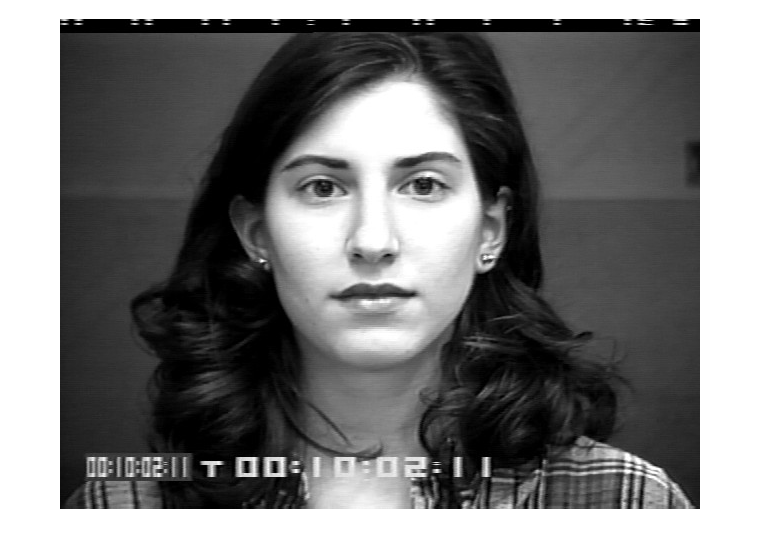
\includegraphics[scale=.10]{figure/77/04.png}
    	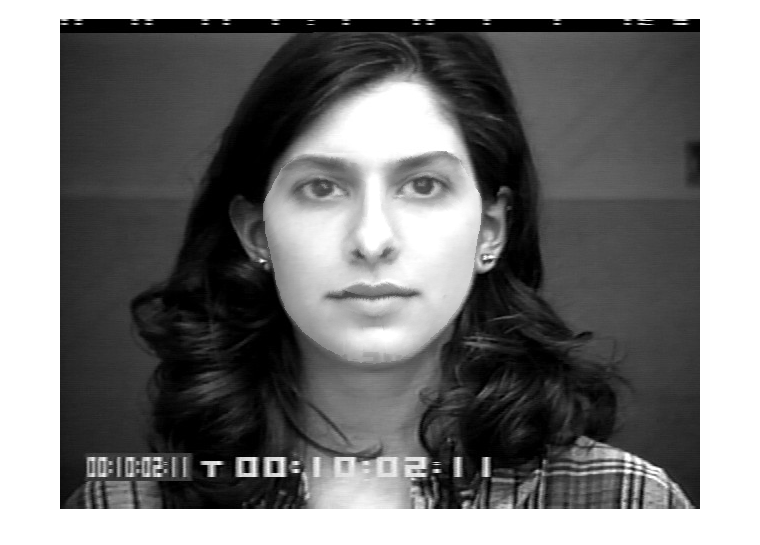
\includegraphics[scale=.10]{figure/77de/04.png}
    	\hspace{1cm}
    	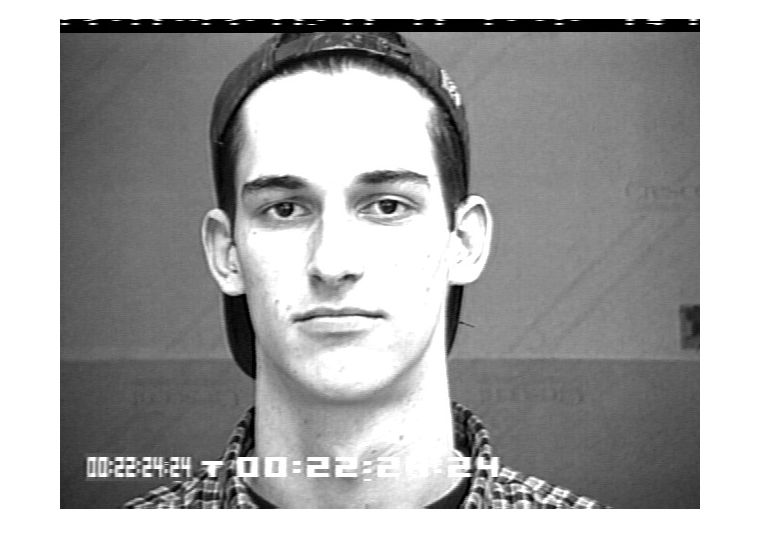
\includegraphics[scale=.10]{figure/89/05.png}
    	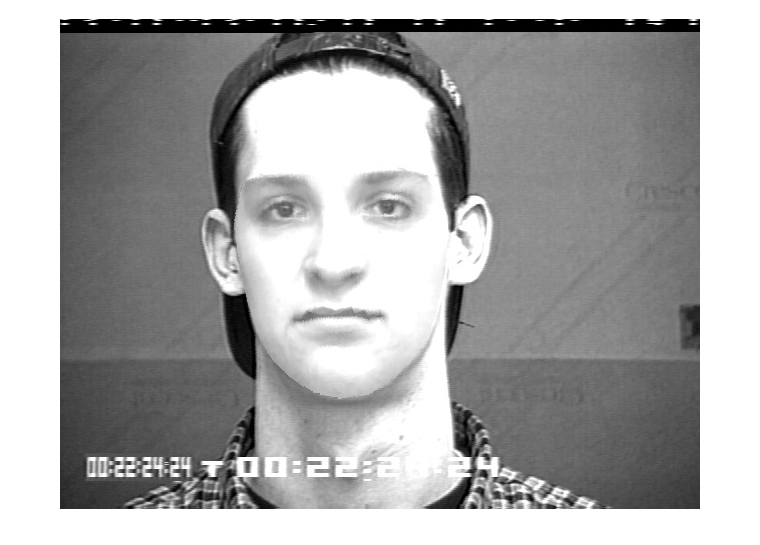
\includegraphics[scale=.10]{figure/89de/05.png}

    	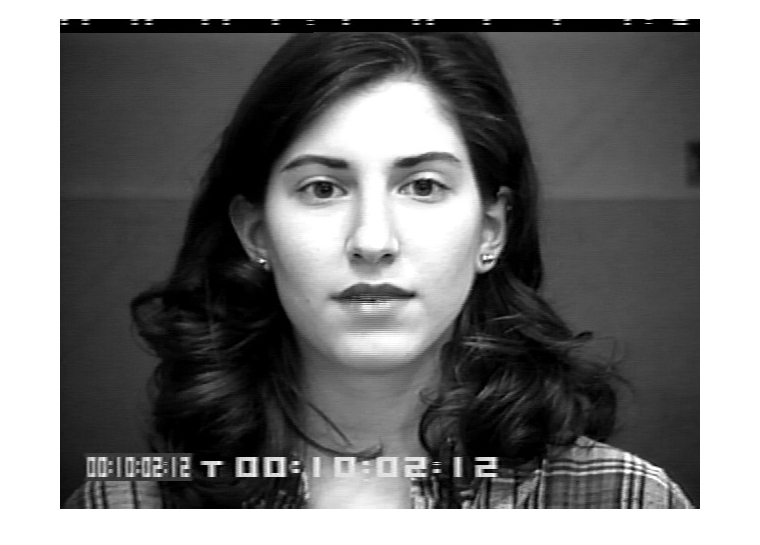
\includegraphics[scale=.10]{figure/77/05.png}
    	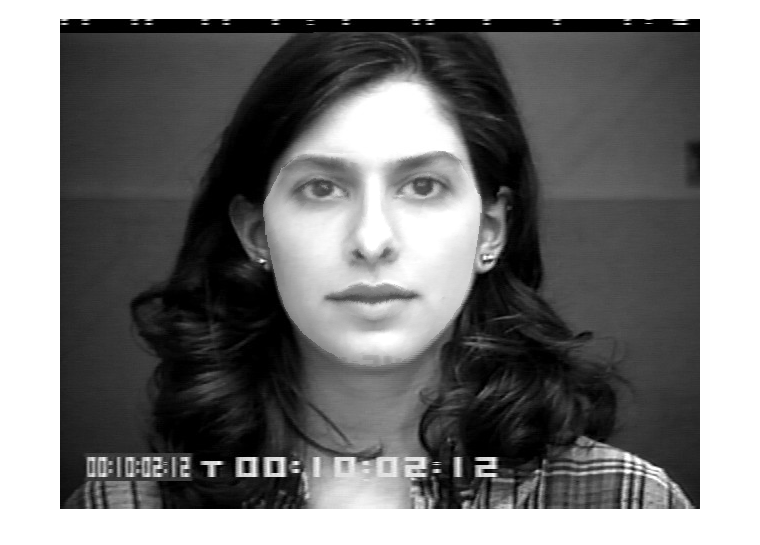
\includegraphics[scale=.10]{figure/77de/05.png}
    	\hspace{1cm}
    	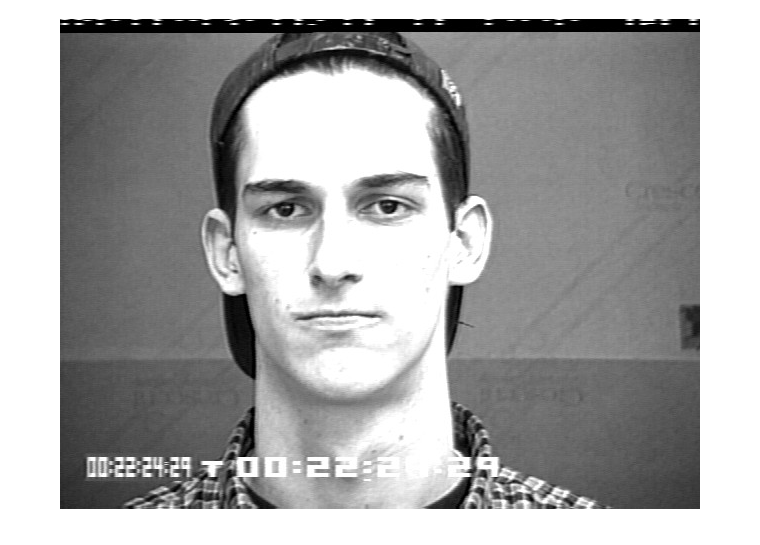
\includegraphics[scale=.10]{figure/89/10.png}
    	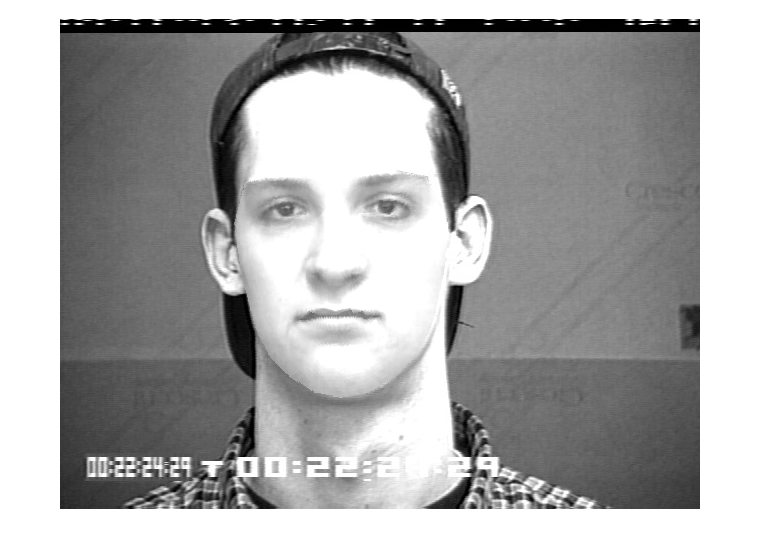
\includegraphics[scale=.10]{figure/89de/10.png}

    	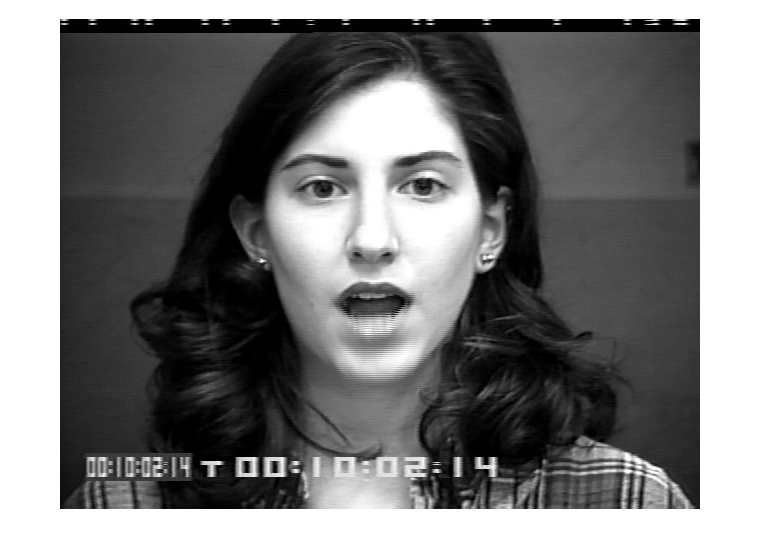
\includegraphics[scale=.10]{figure/77/07.png}
    	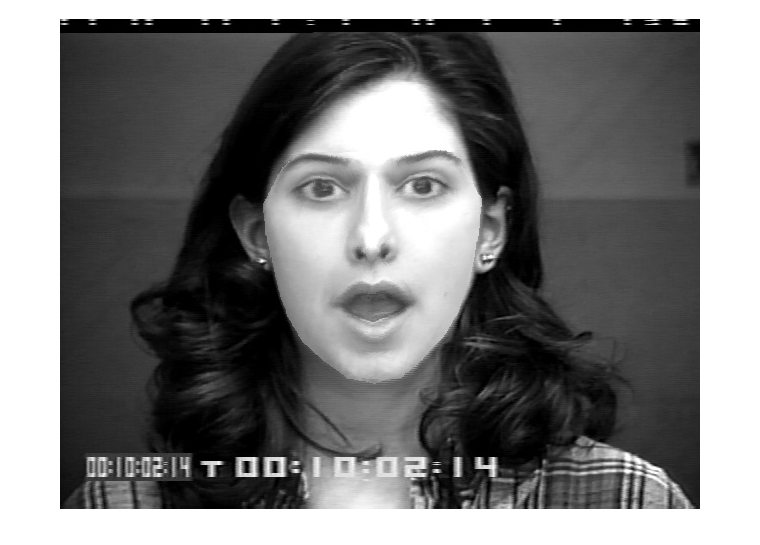
\includegraphics[scale=.10]{figure/77de/07.png}
    	\hspace{1cm}
    	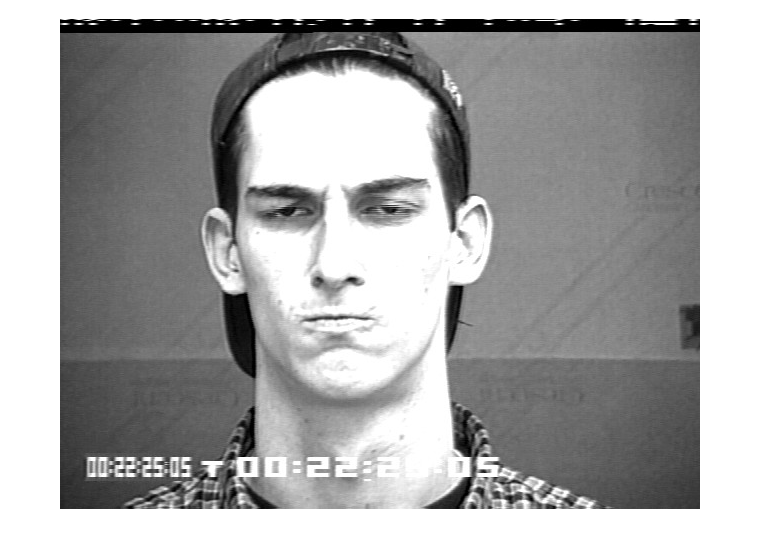
\includegraphics[scale=.10]{figure/89/16.png}
    	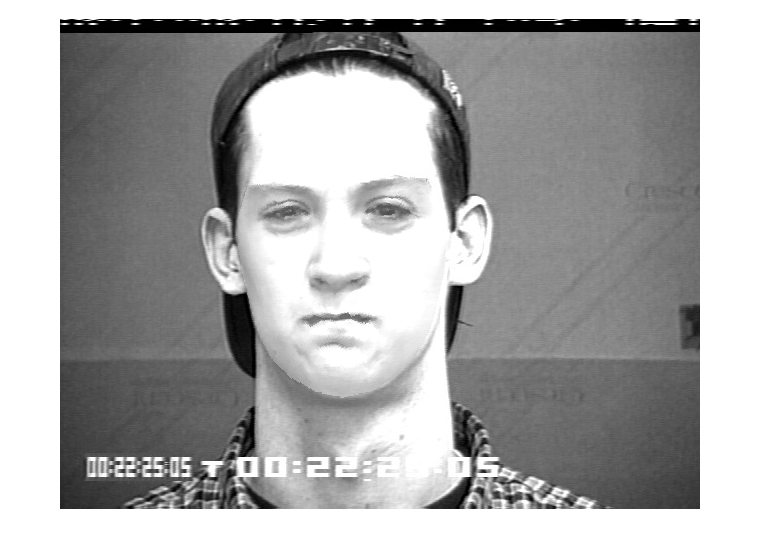
\includegraphics[scale=.10]{figure/89de/16.png}

    	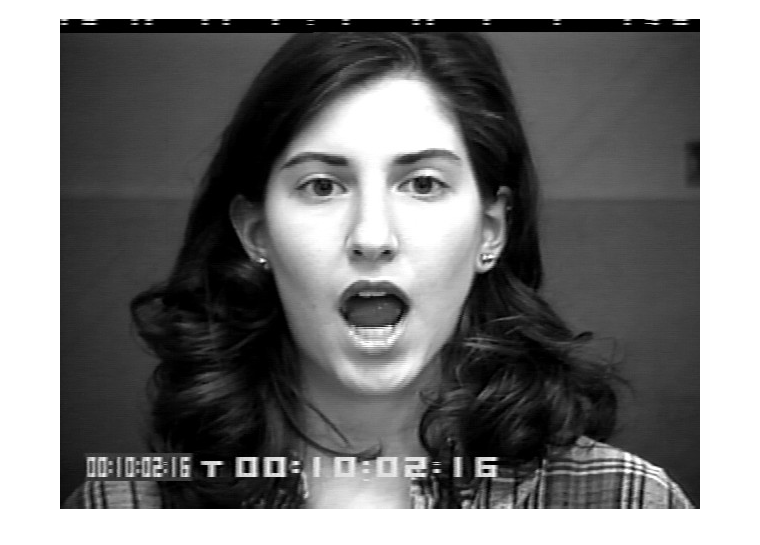
\includegraphics[scale=.10]{figure/77/09.png}
    	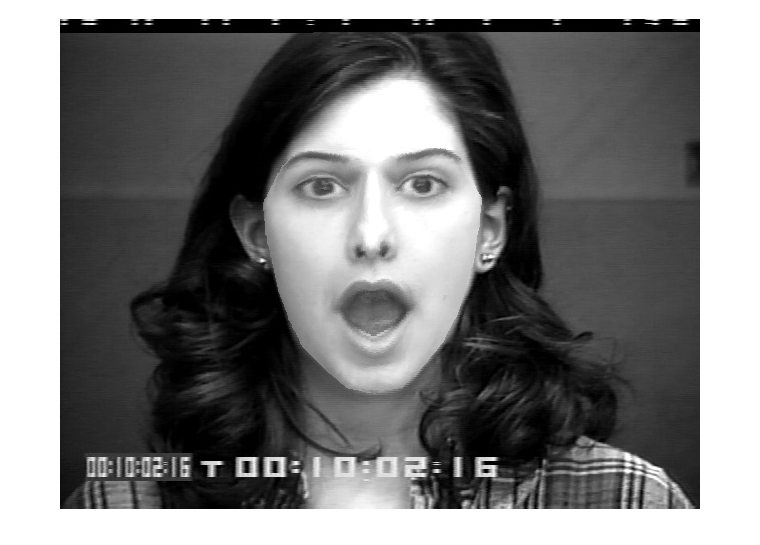
\includegraphics[scale=.10]{figure/77de/09.png}
    	\hspace{1cm}
    	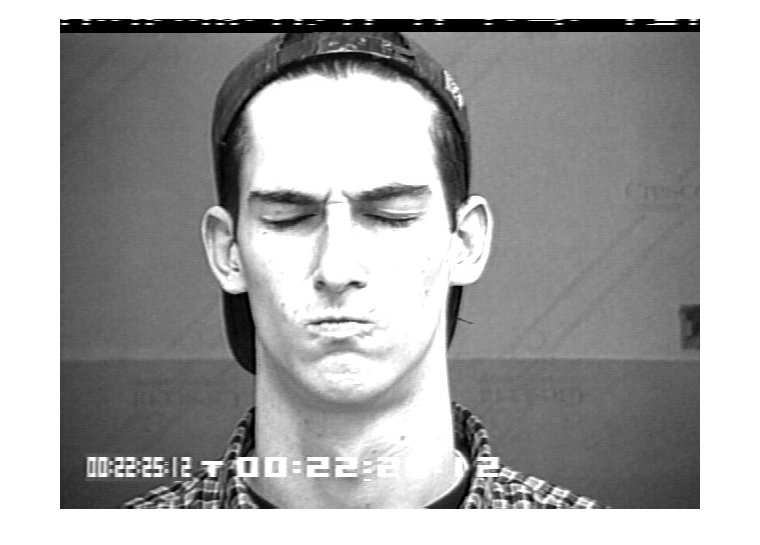
\includegraphics[scale=.10]{figure/89/23.png}
    	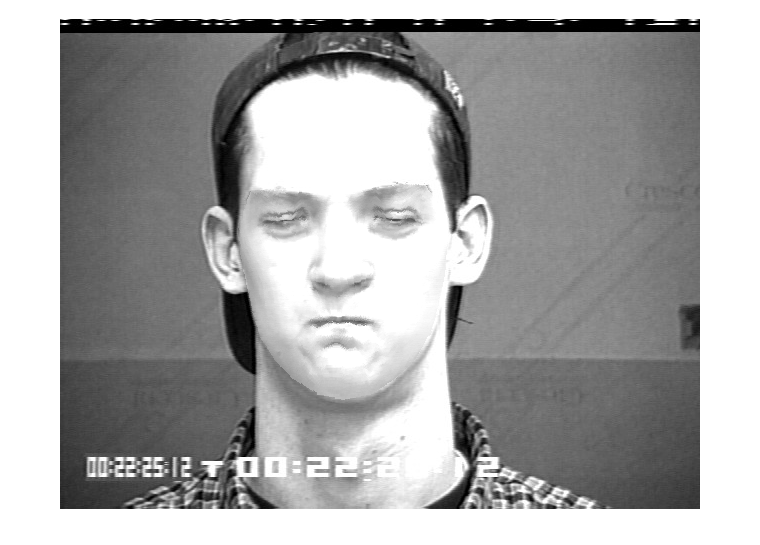
\includegraphics[scale=.10]{figure/89de/23.png}

    	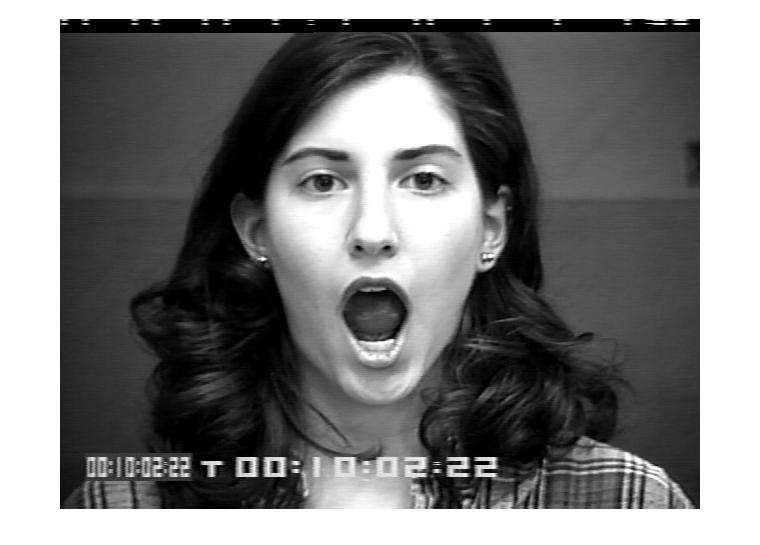
\includegraphics[scale=.10]{figure/77/15.png}
    	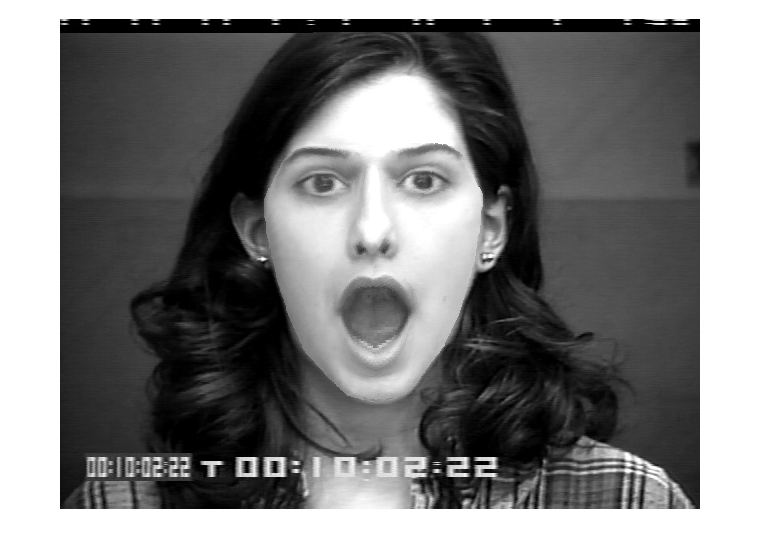
\includegraphics[scale=.10]{figure/77de/15.png}
    	\hspace{1cm}
    	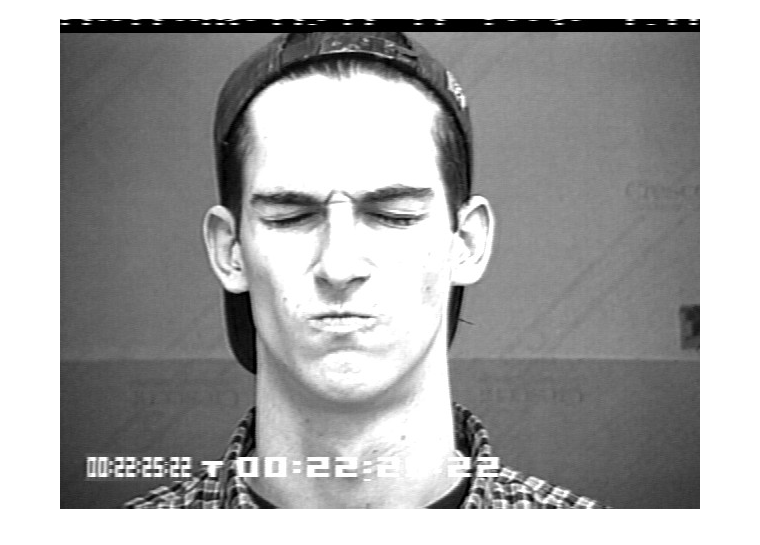
\includegraphics[scale=.10]{figure/89/33.png}
    	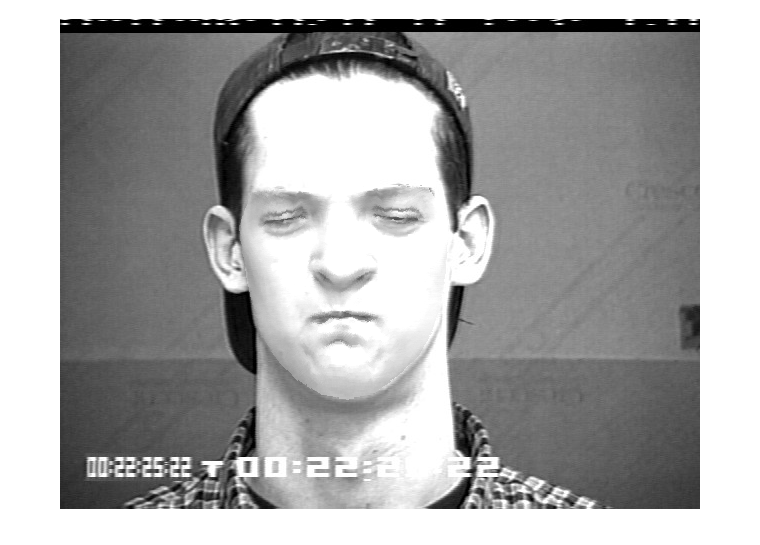
\includegraphics[scale=.10]{figure/89de/33.png}

		\caption{ $k=2$. Each column is a series of frames from a video. The first column is the series of
		original frames with surprise expression, and the third column is the original ones with anger expression.  
		The second and fourth columns are the de-identified frames respectively.}
		\label{fig:results}
  	\end{figure}

  	Our pre-processed tensor did not involve the factors about skin colors. Therefore, in order to make the de-identified
  	images more natural, the final result
  	adds the value of the difference between the mean of original textures and the mean of de-identified
  	results. Two more results on neutral and happy expressions are illustrated in Fig. \ref{fig:results_2}. 
  	As the results demonstrated, we can claim that our algorithm is able to de-identify a series of frames
  	in a video with natural results and keep the de-identified identity invariant. Meanwhile, the proposed
  	algorithm could fully protect the original data utilities, such as expressions. 


	\begin{figure}[!htb]
    	\centering
    	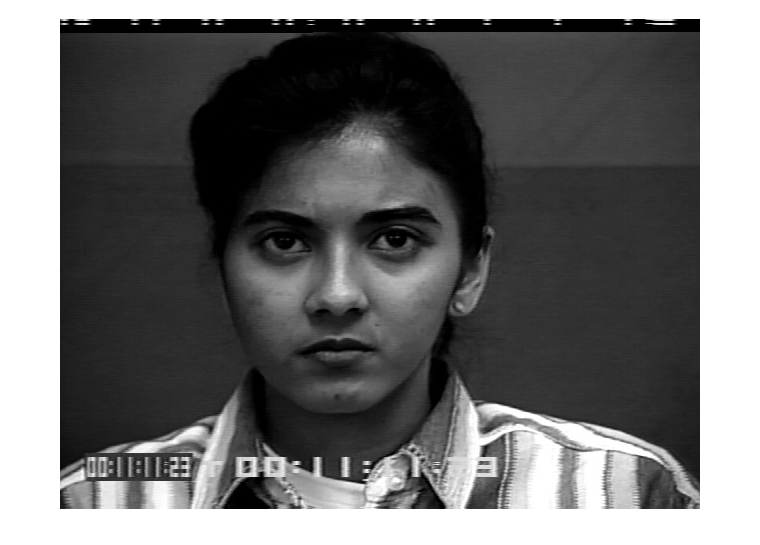
\includegraphics[scale=.10]{figure/79/01.png}
    	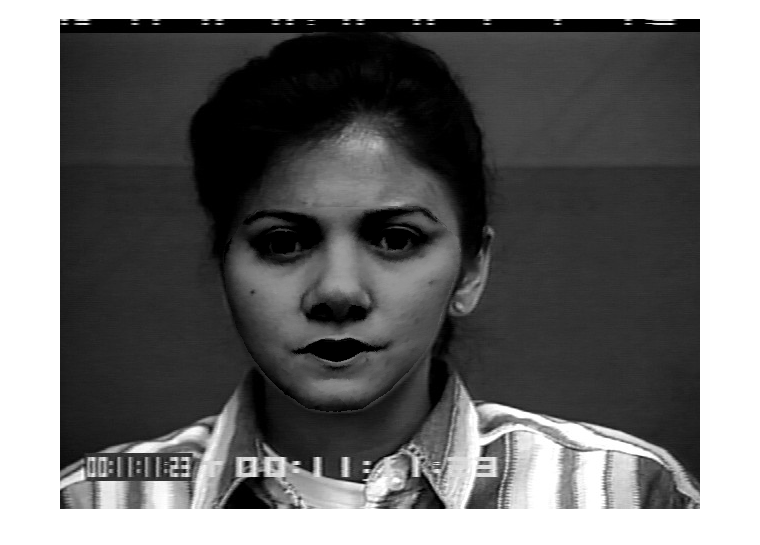
\includegraphics[scale=.10]{figure/79de/01.png}
    	\hspace{1cm}
    	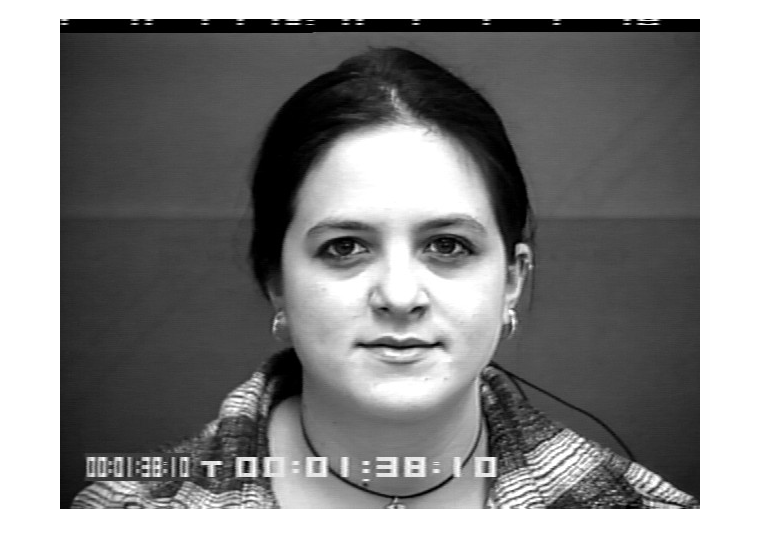
\includegraphics[scale=.10]{figure/72/02.png}
    	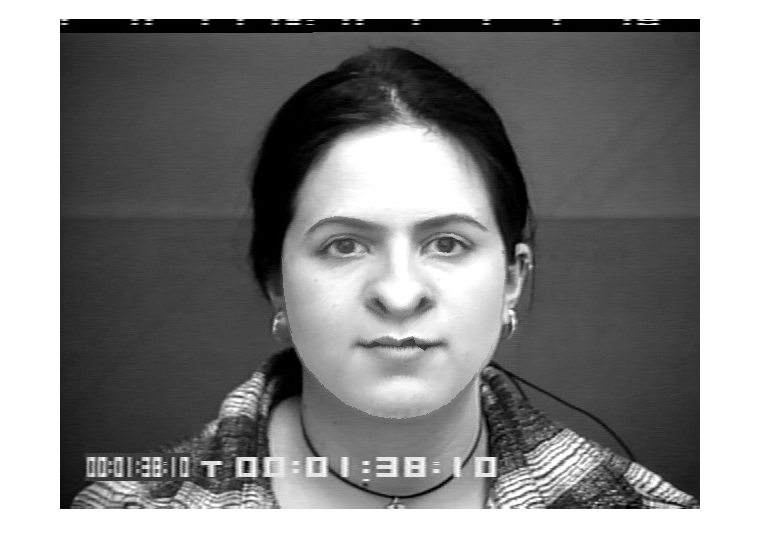
\includegraphics[scale=.10]{figure/72de/02.png}

    	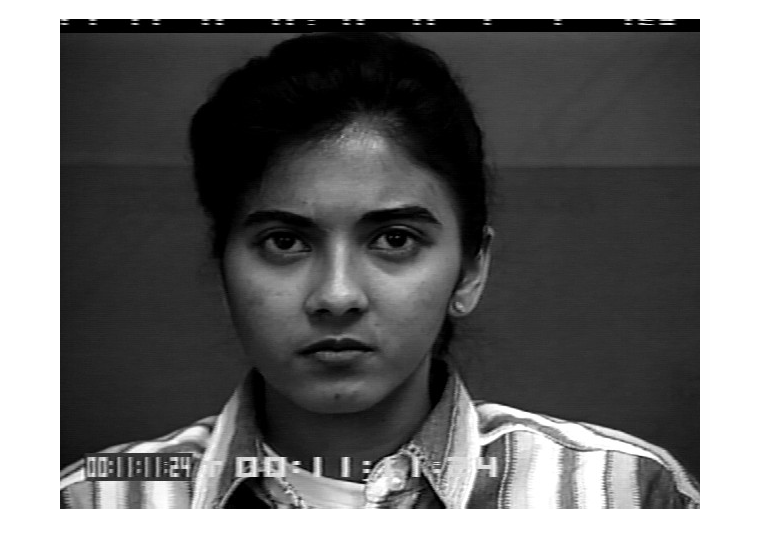
\includegraphics[scale=.10]{figure/79/02.png}
    	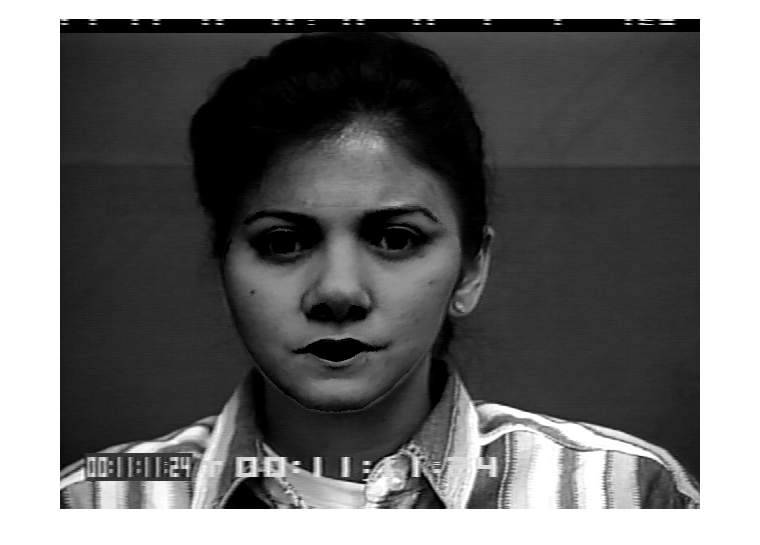
\includegraphics[scale=.10]{figure/79de/02.png}
    	\hspace{1cm}
    	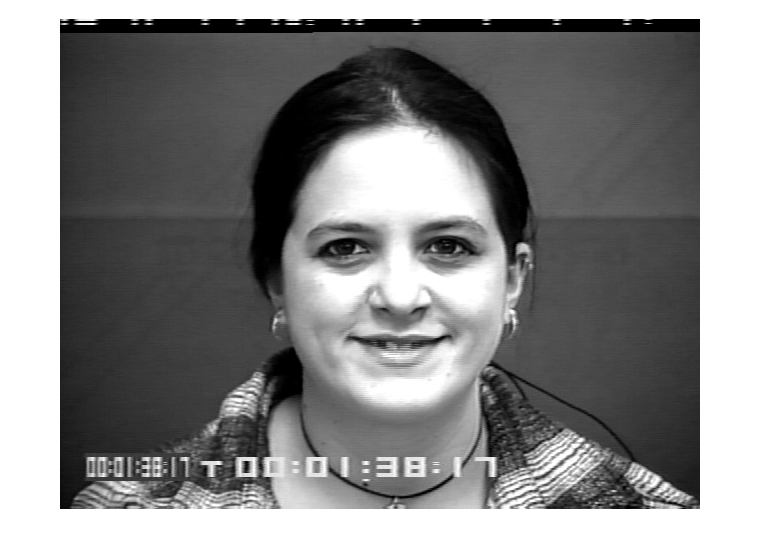
\includegraphics[scale=.10]{figure/72/09.png}
    	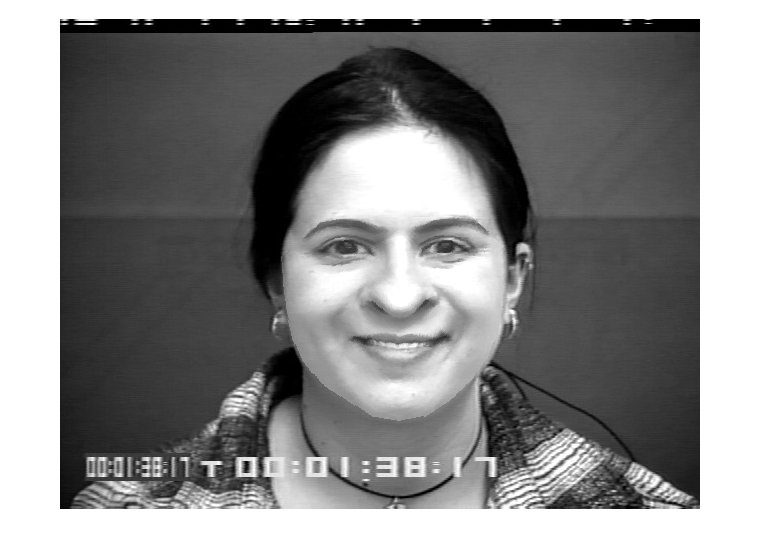
\includegraphics[scale=.10]{figure/72de/09.png}

    	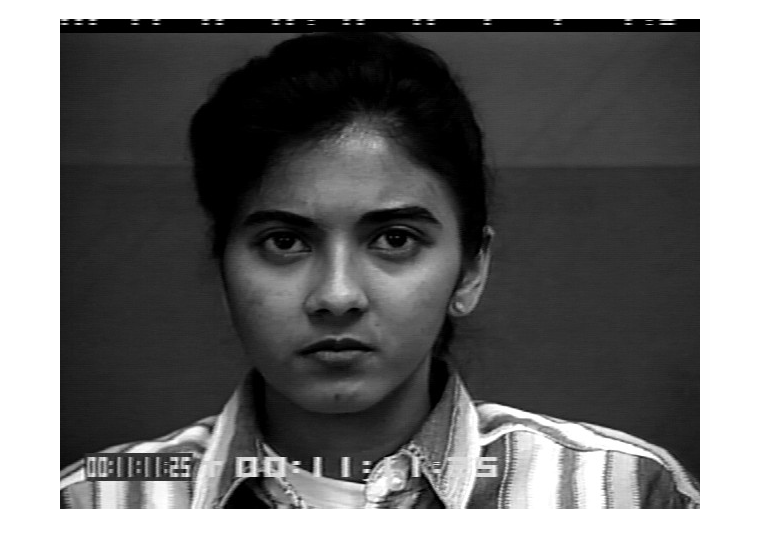
\includegraphics[scale=.10]{figure/79/03.png}
    	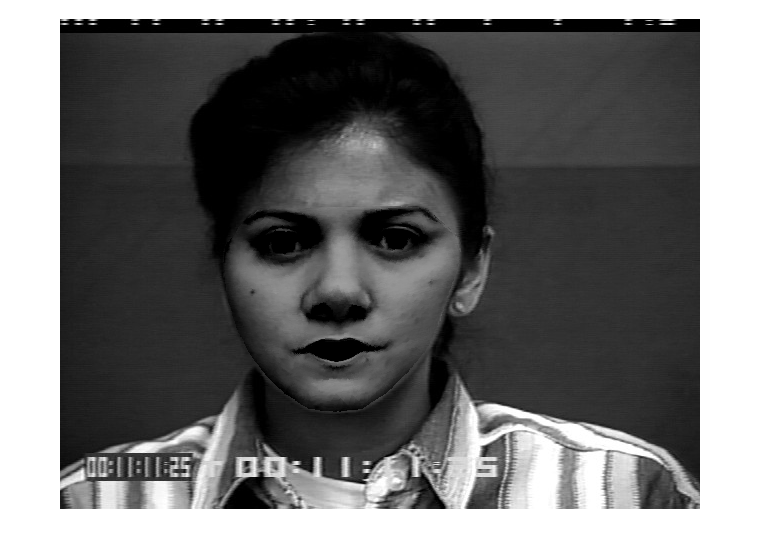
\includegraphics[scale=.10]{figure/79de/03.png}
    	\hspace{1cm}
    	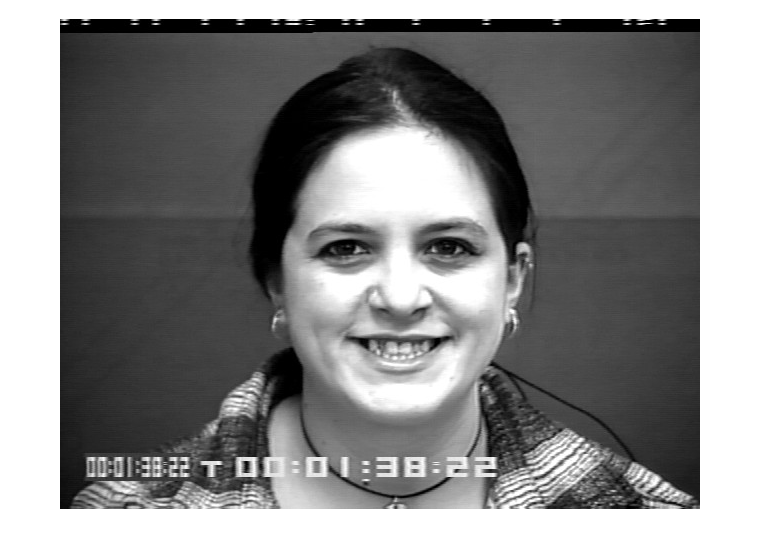
\includegraphics[scale=.10]{figure/72/14.png}
    	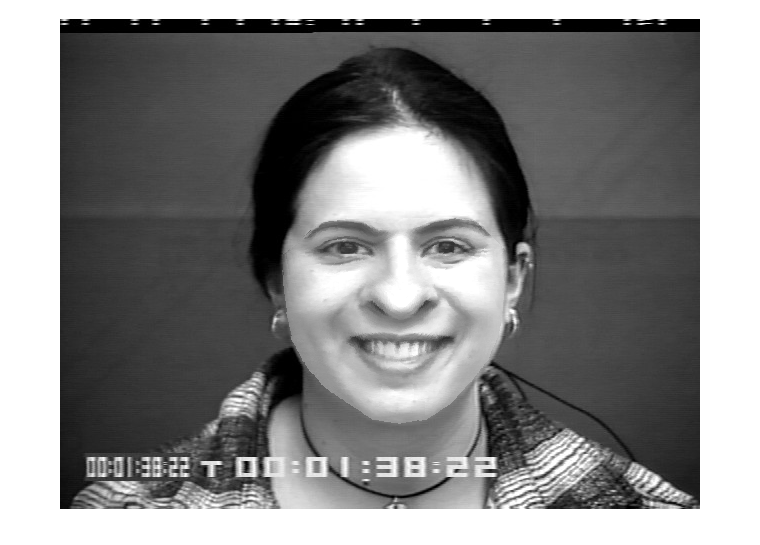
\includegraphics[scale=.10]{figure/72de/14.png}

		\caption{ De-identified images of different subjects with neutral and happy expressions. $k=5$. The 
		first and third columns are the original frames. The second and fourth columns are the 
		de-identified resutls respectively. }
		\label{fig:results_2}
  	\end{figure}




We can quantify the similarity between the original frames and the de-identified results using the comparison 
demo, which is supplied by OpenFace \cite{facenet15,openface16} and outputs the predicted similarity score of two faces by 
computing the squared L2 distance between their model representations.


	\begin{figure}[!htb]
    	\centering
    	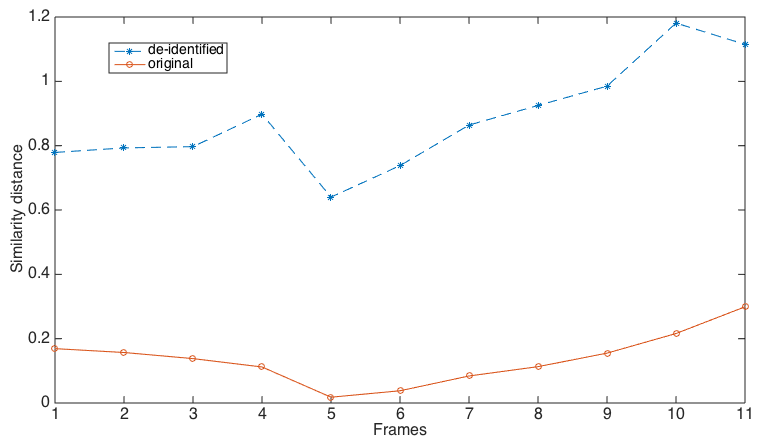
\includegraphics[width=14cm]{figure/distance.png}
    	
		\caption{ Similarity distance. Red solid line: similarity distance between de-identified frames and the target frame.
				  Blue dash line: similarity distance between original frames and the target frame.}
		\label{fig:distance}
  	\end{figure}
The left subject shown in Fig. \ref{fig:results} is taken for example. Eleven original frames and the corresponding
de-identified frames are picked out, and one de-identified frame is randomly chosen as a target frame. The similarity 
between the original \& de-identified frames and the target frame is shown in
Fig. \ref{fig:distance}. Seen from the figure,
the de-identified frames are obvious more close to the target frame. Furthermore, the distances between
de-identified results are small. 